\documentclass{tufte-handout}

%\geometry{showframe}% for debugging purposes -- displays the margins

\usepackage{amsmath}
\usepackage{amssymb}
\usepackage{amsthm}
\usepackage{thmtools}

\declaretheorem[numberwithin=section]
{theorem, definition}
\declaretheorem{lemma, proposition, corollary}[
style=plain,
numberwithin=theorem
]
% Set up the images/graphics package
\usepackage{graphicx}
\setkeys{Gin}{width=\linewidth,totalheight=\textheight,keepaspectratio}
\graphicspath{{graphics/}}
\usepackage{float}

\title{MATH 350 Notes}
\author{Shan Gao}
\date{Fall 2023}

% The following package makes prettier tables.  We're all about the bling!
\usepackage{booktabs}

% The units package provides nice, non-stacked fractions and better spacing
% for units.
\usepackage{units}

% The fancyvrb package lets us customize the formatting of verbatim
% environments.  We use a slightly smaller font.
\usepackage{fancyvrb}
\fvset{fontsize=\normalsize}

% Small sections of multiple columns
\usepackage{multicol}

% Provides paragraphs of dummy text
\usepackage{lipsum}

% These commands are used to pretty-print LaTeX commands
\newcommand{\doccmd}[1]{\texttt{\textbackslash#1}}% command name -- adds backslash automatically
\newcommand{\docopt}[1]{\ensuremath{\langle}\textrm{\textit{#1}}\ensuremath{\rangle}}% optional command argument
\newcommand{\docarg}[1]{\textrm{\textit{#1}}}% (required) command argument
\newenvironment{docspec}{\begin{quote}\noindent}{\end{quote}}% command specification environment
\newcommand{\docenv}[1]{\textsf{#1}}% environment name
\newcommand{\docpkg}[1]{\texttt{#1}}% package name
\newcommand{\doccls}[1]{\texttt{#1}}% document class name
\newcommand{\docclsopt}[1]{\texttt{#1}}% document class option name


\begin{document}
\maketitle
\begin{abstract}
	Collection of personal notes  
\end{abstract}
\section{Lecture 1 : Introduction}
The main study of this class is of graph theory. 
\begin{definition}[Graph]
	A graph $G$ consist of a set of \textbf{vertices} denoted by $V(G)$ and some pairs of vertices called \textbf{edges}, denoted by $E(G)$. It is clear that $E(G) \subseteq V(G) \times V(G)$. In this class $E(G)$ and $V(G)$ will always be finite.  	
\end{definition}
\begin{definition}[adjacent]
	$2$, vertices, $u,v \in V(G)$ are \textbf{adjacent} if $(u,v) \in E(G)$. 

\end{definition}
We state a problem involving Graphs. This is the Koninsberg bridge problem, solved by Euler in 1735. We have 2 islands joined to each other and to the shores by 7 bridges, the citizens want to take a stroll along all the islands such that they are crossing each one of the 7 bridges \textbf{once} exactly. The question is: is it possible? We'll skip the fancy diagram with the bridges and shores and move on to the graph representation of this problem. 
\begin{marginfigure}%
	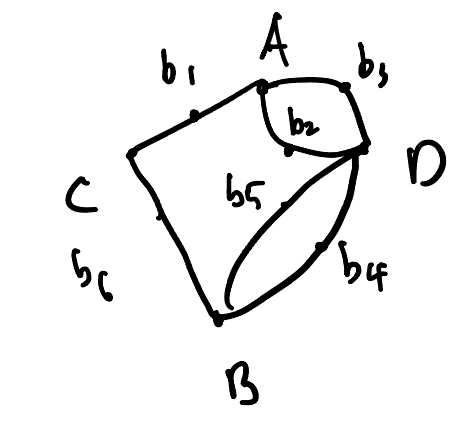
\includegraphics[width=\linewidth]{ex1.jpeg}
	\caption{Graph of problem, minor correction to the graph there is an edge between island $C$ and island $D$}        
	\label{fig:ex1}
\end{marginfigure}
In the uncorrected figure about, there exists an \textbf{Euler Walk}. However if you add an edge $(C,D)$ there does not exist one. The proof is that for a vertex that is neither the start nor the end point of the walk needs to have \textbf{even} degree, since when we enter a vertex, we must exit it. Only the start and endpoints can have odd degree. So the maximum amount of vertices with odd degree is $2$, in the corrected graph there are 4 vertices with odd degree, so a Euler Walk is impossible. In the uncorrected one, we have 2 vertices of odd degree, $C$ and $D$, taking those 2 to be the start and endpoints, it's easy to find a Euler Walk around the graph. 
\begin{theorem}[Ramsey number 3]
	If a graph $G$ with $6$ vertices, there are either a set of 3 pairwise adjacent vertices or a set of 3 pairwise non adjacent vertices. 	
\end{theorem}
the proof is trivial

\end{document}

